\documentclass[a4paper,12pt]{extarticle}
\usepackage[utf8]{inputenc}
\usepackage[T1]{fontenc}
\usepackage[main=english,russian]{babel}
\usepackage{geometry}
\geometry{left=2.5cm,right=1.5cm,top=2cm,bottom=2cm}
\usepackage{url}
\usepackage[strings]{underscore}
\usepackage{enumitem}
\usepackage{amsmath}
\usepackage{amsthm}
\usepackage{amssymb}
\usepackage{fancyhdr}
\usepackage{setspace}
\usepackage{graphicx}
\usepackage{colortbl}
\usepackage{tikz}
\usepackage{pgf}
\usepackage{subcaption}
\usepackage{listings}
\usepackage{indentfirst}
\usepackage[
backend=biber,
style=numeric,
urldate=long,
maxbibnames=99
]{biblatex}
\addbibresource{refs.bib}
\usepackage[colorlinks,citecolor=blue,linkcolor=blue,bookmarks=false,hypertexnames=true,urlcolor=blue]{hyperref}
\usepackage{mathtools}
\usepackage{booktabs}
\usepackage[flushleft]{threeparttable}

\usepackage{chngcntr}
\counterwithin{table}{section}
\counterwithin{figure}{section}

\graphicspath{{graphics/}}

\setlength{\parindent}{1.25cm}
\renewcommand{\baselinestretch}{1.5} % междустрочный интервал


\newcommand{\bibref}[3]{\hyperlink{#1}{#2 (#3)}} 
\addto\captionsrussian{\def\refname{Список литературы (или источников)}} 

\renewcommand{\theenumi}{\arabic{enumi}}%
\renewcommand{\labelenumi}{\arabic{enumi}}%
\renewcommand{\theenumii}{.\arabic{enumii}}%
\renewcommand{\labelenumii}{\arabic{enumi}.\arabic{enumii}.}%
\renewcommand{\theenumiii}{.\arabic{enumiii}}%
\renewcommand{\labelenumiii}{\arabic{enumi}.\arabic{enumii}.\arabic{enumiii}.}%

\begin{document}
\begin{titlepage}
\newpage

{\setstretch{1.0}
\begin{center}
NATIONAL RESEARCH UNIVERSITY\\
HIGHER SCHOOL OF ECONOMICS
\\
\bigskip
Faculty of Computer Science\\
Bachelor’s Programme “Data Science and Business Analytics”
\end{center}
}

\vspace{2em}

\vspace{4em}

\begin{center}
%Выберите какой у вас проект
{\bf Software Project Report on the Topic:}\\
%{\bf Research Team Project Report on the Topic:}\\
%{\bf Software Project Report on the Topic:}\\
%{\bf Software Team Project Report on the Topic:}\\
{\bf Analytical System for the Interdependence of Ruble and Yuan Borrowing Rates: Macroeconomic Drivers and Arbitrage Potential}\\
% строчка ниже нужна только при сдача плана КР, при финальной сдаче закомментируйте ее
(interim, the first stage)
\end{center}

\vspace{2em}

{\bf Submitted by the Student: \vspace{2mm}}
%{\bf Submitted by the Students: \vspace{2mm}}

{\setstretch{1.1}
\begin{tabular}{l@{\hskip 1.5cm}l}
group \#\foreignlanguage{russian}{БПАД}231, 3rd year of study & 
Sotova Veronika Konstantinovna \\
%group \#\foreignlanguage{russian}{БПМИ}191, 3th year of study & Ivanov Dmitrii Mikhailovich \\
\end{tabular}}

% Обычно у вас есть один научный руководитель, и это человек, с которым вы работаете над проектом. Иногда по формальным причинам у вас будет руководитель (штатный сотрудник Вышки) и соруководитель (тот, с кем вы работаете), — об этом вам сообщит учебный офис (в случае с ВКР) или ЦППРиП (в случае с курсовым проектом). Также, если кто-то дополнительно вам помогал, то его можно указать как консультанта. 

%ваш официальный научник (из ВШЭ)
\vspace{1em}
{\bf Approved by the Project Supervisor: \vspace{2mm}}

{\setstretch{1.1}
\begin{tabular}{l@{\hskip 1.5cm}l}
Potapov Ivan Andreevich\\
Senior Software Engineer\\
Zelando SE
\end{tabular}}

% со-руководитель (если есть)
%\vspace{1em}
%{\bf Co-supervisor: \vspace{2mm}}

%{\setstretch{1.1}
%\begin{tabular}{l@{\hskip 1.5cm}l}
%Petrova Ekaterina Maksimovna\\
%Research Fellow\\
%AO "Neural networks in the wild" 
%\end{tabular}}

% консультант (если есть)
%\vspace{1em}
%{\bf Consultant: \vspace{2mm}}

%{\setstretch{1.1}
%\begin{tabular}{l@{\hskip 1.5cm}l}
%Ivanova Ekaterina Maksimovna\\
%Research Fellow\\
%AO "Neural networks in the wild" 
%\end{tabular}}

\vspace{\fill}

\begin{center}
Moscow 2026
\end{center}

\end{titlepage}%
\newpage
\setcounter{page}{2}

{
	\hypersetup{linkcolor=black}
	\tableofcontents
}

\newpage

\newpage
\section*{Annotation} 
\addcontentsline{toc}{section}{Annotation}

This project develops an end-to-end system that connects the analysis of Ruble and Yuan borrowing rates to executable, governance-constrained portfolio decisions. The goal is to identify relative-value opportunities and maximise risk-adjusted return subject to VaR, liquidity, turnover, and reproducibility constraints. The implemented stack combines: (i) a modular data pipeline (CBR, MOEX, FRED, AKShare, ChinaBond), (ii) statistical analysis of RUB/CNY interdependence, (iii) forecasting baselines and spread diagnostics, (iv) an arbitrage signal layer with triple-barrier/meta-labeling and ML classifiers, (v) regime smoothing with Markov-switching probabilities and persistence filters, and (vi) a confidence-weighted router with explicit no-trade reasons. Reliability and robustness diagnostics (Brier/reliability bins, threshold/cost stability grids, artifact schema checks) are included in the current workflow. AER remains an extension, while regime-aware decisioning and risk-aware backtests are already operational in the current implementation.

\section*{\foreignlanguage{russian}{Аннотация}}
\foreignlanguage{russian}{
Проект разрабатывает сквозную систему, связывающую анализ ставок заимствования рубля и юаня с исполняемыми портфельными решениями при ограничениях риска и воспроизводимости. Реализованы: конвейер данных (ChinaBond \texttt{load\_from\_directory()}, FRED API), \texttt{StatisticalAnalyzer} (описательная статистика, корреляция, стационарность, коинтеграция, Грейнджер, VAR, OLS), блок прогнозирования и сигналов (NS-подгонка, кросс-валютные спреды, triple-barrier/meta-labeling, ML-классификаторы), сглаживание режимов (Markov-switching с фильтром устойчивости), а также confidence-weighted роутер с причинами no-trade. Добавлены диагностические контуры надёжности и устойчивости (Brier/reliability, sensitivity grids). AER сохраняется как расширение, тогда как режимно-осведомлённые решения и риск-учитывающие бэктесты уже внедрены.
}

\section*{Keywords}
\noindent RUB/CNY borrowing rates; relative-value opportunities; arbitrage identification; yield-curve modeling; Nelson--Siegel; portfolio optimization; VaR constraints; data pipeline; statistical analysis; cross-currency spreads.

\pagebreak

\section{Introduction}

Ruble and Yuan borrowing rates are key price signals for investors, issuers, and policy observers. In both markets, the yield curve reflects domestic macro policy, inflation expectations, liquidity conditions, and international transmission channels. These channels generate nontrivial co-movements between RUB and CNY term structures, but they also create temporary dislocations across maturities and currencies. In practice, analysts often need a reproducible way to detect such dislocations and evaluate whether they are economically meaningful after costs and risk controls.

Despite significant progress in yield-curve modeling, operational workflows are often fragmented: one stack for data collection, another for forecasting diagnostics, and a separate layer for strategy testing. This fragmentation weakens traceability and makes it harder to compare methods under a consistent out-of-sample protocol. The present project addresses this practical gap in the RUB/CNY fixed-income setting by implementing an end-to-end system that links data ingestion, signal generation, regime handling, decision routing, and backtest/inference reporting in one artifact-driven pipeline.

\subsection{Motivation and background}

The identification of arbitrage opportunities in fixed-income markets remains a central problem. No-arbitrage models are designed to describe internally coherent curves, but market data still contain frictions, delayed adjustment, and cross-market imbalances. This raises a practical question: can model residuals, spread deviations, and regime-conditioned dynamics be used as reliable decision inputs in a controlled strategy framework?

For RUB/CNY markets, this question is especially relevant. The environment combines heterogeneous policy regimes, uneven data coverage across sources, and non-negligible transaction frictions. A method that looks promising in isolated statistical diagnostics may fail once costs, turnover, and confidence thresholds are applied. Therefore, the project is motivated not only by forecasting quality, but by the need to convert forecasting outputs into transparent and risk-aware decisions.

\subsection{Scope and objective}

Formally, this coursework is a software project with analytical validation. The scope is to design and evaluate a reproducible decision-support system for relative-value and arbitrage-style detection in RUB/CNY fixed-income data. The system integrates classical and ML signal families, regime labeling, and routing rules under explicit operational constraints.

The core objectives are:
\begin{enumerate}[leftmargin=*, itemsep=0.3em]
\item \textbf{Comparative evaluation.} Run a consistent out-of-sample comparison of implemented classical and ML approaches, and assess not only economic metrics but also inference and robustness diagnostics.
\item \textbf{Arbitrage signal system.} Convert forecasting and spread outputs (residuals, z-score spread deviations, regime-conditioned behavior) into structured monthly signals.
\item \textbf{Decision routing and governance.} Apply confidence/expected-edge gates, disagreement checks, and regime conflict logic to produce auditable trade/no-trade decisions with reason codes.
\item \textbf{Portfolio-level validation.} Evaluate outputs with cost-aware backtests, turnover diagnostics, and statistical inference so that conclusions are conservative and traceable.
\end{enumerate}

\subsection{Relevance and practical significance}

The project has both methodological and practical value. Methodologically, it shows how to combine labeling discipline (triple-barrier and meta-targets), leakage-aware validation (purged/embargo scheme), calibration/stability checks, and regime-aware routing in one coherent workflow. Practically, it provides an operator-facing decision chain with explicit fields (\texttt{selected\_model}, \texttt{confidence}, \texttt{expected\_net\_edge}, \texttt{reason\_code}, \texttt{no\_trade}) and unified decision exports for monthly review.

For applied use, this matters because profitability claims in this domain are highly sensitive to sampling, costs, and thresholds. A reproducible process with schema-checked artifacts and explicit claim governance is more valuable than isolated point estimates. The framework is therefore intended as a controlled decision-support prototype rather than an unconditional alpha claim.

\subsection{Current stage}

At the current stage, the following components are implemented in the repository:
\begin{itemize}
\item \textbf{Data pipeline.} Modular ingestion from CBR, MOEX, FRED, AKShare, and manual ChinaBond sources with SQLite persistence and monthly-aligned panels.
\item \textbf{Statistical layer.} Descriptive statistics, correlation analysis, stationarity/cointegration diagnostics, Granger causality, VAR, and OLS artifacts.
\item \textbf{Yield-curve and spread baseline.} Nelson--Siegel fitting for RU/CN curves, residual diagnostics, matched-maturity RUB--CNY spreads, and abnormal spread flags.
\item \textbf{ML signal layer.} Triple-barrier labels, meta-target construction, walk-forward training with purged/embargo logic, and multi-model probability outputs.
\item \textbf{Regime and routing layer.} Rule-based regimes, Markov-smoothed states with persistence filtering, lagged causal usage, and confidence-weighted decision routing with reason codes.
\item \textbf{Evaluation and reporting.} Classical/ML/regime/unified backtests, cost and turnover diagnostics, bootstrap/paired-test inference, schema checks, and notebook-based reproducible demo flow.
\end{itemize}

At the same time, some extensions remain outside the current production scope, including full AER integration in an HJM-consistent framework and a fuller optimizer layer with richer forward-looking risk engines.

\subsection{Structure of the report}

The rest of the report is organized as follows. Section 2 positions the project relative to key literature strands. Section 3 describes implemented system design and module interfaces. Section 4 defines the validation protocol and interpretation rules. Section 5 summarizes evidence from exported artifacts with conservative claim governance. Section 6 discusses practical use, limits, and next steps. Section 7 concludes. Detailed diagnostics and extended tables are provided in appendices.

\pagebreak

\section{Analogue and Literature Positioning}

\subsection{Yield curve modeling and borrowing-rate forecasting}

Recent work on interest-rate modeling shows that machine-learning methods can support nonlinear yield-curve estimation and forecasting \cite{delucchi2025, bluwstein2020}. Tree-based macroeconomic regime switching \cite{bie2025} combines DNS-style term-structure modeling with macro splits (for example, policy-rate and inflation regimes), improving interpretability of regime behavior. Arbitrage-aware filtering frameworks \cite{gao2025} incorporate HJM-consistent constraints and show that Arbitrage Error Regularization (AER) can improve short-end forecast and execution-relevant quality metrics.

\textbf{Gap.} Most yield-curve studies focus on forecast accuracy or monitoring quality rather than direct arbitrage-potential extraction from model residuals/spreads. Applications to RUB/CNY with explicit cross-currency and regime-aware decision layers remain limited relative to developed-market studies.

\subsection{Risk management and scenario evaluation}

Existing work covers Monte Carlo scenario engines for return-distribution estimation \cite{celestin2025}, static vs dynamic dependence diagnostics (including DCC/GARCH-type ideas) for regime shifts \cite{vasuki2025}, and ML-assisted risk prediction for risk-adjusted outcomes \cite{uddin2025}.

\textbf{Gap.} Risk modules are frequently treated as standalone diagnostics rather than integrated controls linked to monthly signal gating, turnover/cost accounting, and final model routing in one reproducible pipeline.

\subsection{Portfolio optimization and decision engines}

Portfolio decision-engine research includes DRL-based dynamic allocation with risk-adjusted rewards \cite{huang2024}, deployment-oriented AI portfolio stacks with temporal models and uncertainty control \cite{suratwala2025}, sparse selection under dependence \cite{machkour2025}, and ML-vs-classical allocation comparisons under volatility \cite{olanrewaju2025}.

\textbf{Gap.} Many studies optimize decision engines in isolation and on different asset universes, without integrating policy/macro transmission inputs, yield-curve arbitrage diagnostics, and explicit cost-aware routing constraints in a single operational workflow.

\subsection{This project's contribution}

The contribution of this project is an implemented hybrid software+analytical system that focuses on arbitrage identification (parametric residuals and cross-currency spreads), enriches signals with ML opportunity/direction logic, and produces risk-aware routed decisions under explicit transaction-cost and governance constraints in the RUB/CNY fixed-income setting. By combining cross-currency spread logic, regime persistence handling, and conservative inference framing in one reproducible artifact pipeline, the project addresses a practical integration gap not directly covered by individual literature strands.

\textbf{Section summary.} The literature supports each component separately; the project contribution is their integrated, auditable implementation for the RUB/CNY arbitrage workflow.

\section{System Design and Implementation}

\subsection{System rationale and architecture}

The system is designed as a modular pipeline:
\[
\text{Data ingestion} \to \text{Feature/label construction} \to \text{Signal generation} \to \text{Regime-aware routing} \to \text{Backtest/inference artifacts}.
\]
This architecture supports reproducibility and selective replacement of components without rewriting the full workflow.

\begin{figure}[htbp]
\centering
\begin{tikzpicture}[font=\small]
  \node[draw, align=center, text width=2.5cm] (d) at (0,0) {Data sources\\CBR/MOEX/FRED\\AKShare/ChinaBond};
  \node[draw, align=center, text width=2.3cm] (f) at (3.2,0) {Features\\and labels};
  \node[draw, align=center, text width=2.3cm] (s) at (6.4,0) {Classical + ML\\signals};
  \node[draw, align=center, text width=2.3cm] (r) at (9.6,0) {Regime +\\decision routers};
  \node[draw, align=center, text width=2.5cm] (b) at (12.8,0) {Backtests +\\inference +\\exports};

  \draw[->] (d) -- (f);
  \draw[->] (f) -- (s);
  \draw[->] (s) -- (r);
  \draw[->] (r) -- (b);
\end{tikzpicture}
\caption{End-to-end software pipeline from ingestion to exported decision/backtest artifacts.}
\label{fig:sys_pipeline}
\end{figure}

Figure~\ref{fig:sys_pipeline} summarizes how modules are chained in production scripts and notebooks. The architecture is intentionally linear at artifact boundaries, so each stage can be validated and replaced independently while preserving downstream contracts.

\subsection{Implemented modules and interfaces}

Core implemented components in the repository:
\begin{itemize}
\item \textbf{Data layer}: CBR, MOEX, FRED, AKShare, and manual ChinaBond ingestion into SQLite.
\item \textbf{Forecasting layer}: Nelson--Siegel fitting, spread diagnostics, and baseline evaluation helpers.
\item \textbf{Signal layer}: classical signals and ML signals with triple-barrier/meta-labeling and walk-forward logic.
\item \textbf{Routing layer}: regime labels, persistence filtering, confidence-weighted selection, reason-coded no-trade logic.
\item \textbf{Evaluation layer}: classical/ML/regime/unified backtests with cost, turnover, and inference outputs.
\item \textbf{Demo layer}: notebook run-control and dashboard flow for reproducible demonstration.
\end{itemize}

\subsection{ML model stack and labeling design}

The implemented ML stack combines four direction classifiers at each walk-forward step: \texttt{LogisticRegression}, \texttt{RandomForestClassifier}, calibrated \texttt{RidgeClassifier}, and \texttt{HistGradientBoostingClassifier}. Their probabilities are aggregated into \texttt{proba\_ensemble}, while opportunity probability is modeled separately and combined into final long/short probabilities (\texttt{proba\_final\_long}, \texttt{proba\_final\_short}) before thresholding.

Target construction uses triple-barrier labeling on monthly return differentials with configured take-profit, stop-loss, and maximum holding horizon. From these labels, meta-targets are built as \texttt{target\_opportunity} and conditional \texttt{target\_direction}. This two-stage target design separates ``whether to trade'' from ``which direction to trade'' in the training pipeline.

To reduce leakage risk in model validation, the implementation records a purged/embargo split scheme (\texttt{purged\_embargo\_kx\_embn}) and removes training observations around each test block according to the embargo window.

\subsection{Versioning and schema governance}

The signal stack exposes explicit artifact versions via \texttt{run\_id\_prefix}, \texttt{label\_version}, \texttt{router\_policy\_version}, and \texttt{feature\_block\_version}. Decision artifacts carry these tags so analytical comparisons remain traceable to a specific labeling/routing/feature policy revision.

Schema regression checks are implemented for core outputs. The guard validates both file presence and required columns for \texttt{ml\_signals.csv}, \texttt{ml\_signals\_decisions.csv}, \texttt{regime\_router\_decisions.csv}, and \texttt{unified\_backtest\_summary.csv}. This prevents silent contract drift between scripts, notebooks, and report tables.

\subsection{Reproducibility and artifact governance}

The implementation uses exported CSV/TEX artifacts for traceability, schema checks for regression protection, and a cache/run-control notebook for fast demo vs full recomputation modes. This report references only repository artifacts generated by these scripts.

\textbf{Section summary.} The software system is implemented as a reproducible, modular pipeline with explicit artifact contracts and demonstrable operation.

\section{Analytical Validation Methodology}

\subsection{Data coverage and constraints}

The system uses monthly-aligned time series from implemented sources. Coverage is strongest for Russian policy/curve data (CBR key rate: 2013--2026; CBR G-curve: 2015--2026; MOEX OFZ yields: 2019--2026) and global macro proxies from FRED (2015--2026). PBOC LPR is available from 1991--2026, while Chinese bond yields from AKShare are limited to approximately 12 months and are supplemented by manual ChinaBond files. Russian macro coverage from FRED is partial and ends in 2022-03.

\begin{figure}[htbp]
\centering
\begin{tikzpicture}[font=\small]
  \node[draw, align=center, text width=2.8cm] (c1) at (0,0) {Constraints\\short CN history\\leakage risk\\cost sensitivity};
  \node[draw, align=center, text width=3.2cm] (c2) at (4.4,0) {Design choices\\NS + spreads\\triple-barrier + meta labels\\purged/embargo CV\\confidence/edge gating};
  \node[draw, align=center, text width=3.0cm] (c3) at (8.8,0) {Expected effects\\interpretability\\lower leakage risk\\more robust decisions};
  \draw[->] (c1) -- (c2);
  \draw[->] (c2) -- (c3);
\end{tikzpicture}
\caption{Method-choice rationale: constraints translated into implemented design choices.}
\label{fig:method_choice}
\end{figure}

Figure~\ref{fig:method_choice} links practical constraints to implemented modeling choices.

\begin{figure}[htbp]
\centering
\begin{tikzpicture}[font=\small]
  \node[draw, align=center, text width=2.6cm] (r0) at (0,0) {Monthly\\return differential};
  \node[draw, align=center, text width=2.8cm] (r1) at (3.5,0) {Triple barrier\\TP / SL / time};
  \node[draw, align=center, text width=3.0cm] (r2) at (7.2,0) {Meta targets\\target\_opportunity\\target\_direction};
  \node[draw, align=center, text width=3.2cm] (r3) at (11.4,0) {Purged/embargo CV\\remove samples around\\test folds};
  \draw[->] (r0) -- (r1);
  \draw[->] (r1) -- (r2);
  \draw[->] (r2) -- (r3);
\end{tikzpicture}
\caption{Labeling and validation schema for leakage-aware ML training.}
\label{fig:label_cv}
\end{figure}

Figure~\ref{fig:label_cv} summarizes the implemented labeling and leakage-control logic.

\subsection{Methods under comparison}

Evaluation uses implemented strategy families already exported by the project scripts:
\begin{itemize}
\item classical signal family (panel/spread-based);
\item ML signal family (ensemble and base learners);
\item regime-aware routing and unified strategy layer.
\end{itemize}

\subsection{Metrics, inference, and robustness protocol}

The protocol uses out-of-sample backtest summaries, cost and turnover accounting, and inference artifacts (bootstrap confidence intervals and paired tests). Reliability and robustness are evaluated with calibration bins, stability grids, and regime-cell diagnostics already exported as tables.

\subsection{Reliability, stability, and drift reading rules}

Reliability is read from calibration bins by comparing predicted probability means (\texttt{p\_mean}) with observed event rates (\texttt{y\_rate}); small calibration gaps indicate better probability alignment. Stability is read from threshold-grid outputs (\texttt{active\_pct}, flip proxy): large swings in activity or frequent sign flips under small threshold changes indicate fragile signal behavior.

Drift monitoring is reported through PSI in \texttt{ml\_signals\_drift.csv}. The implementation flags \texttt{alert=1} when PSI reaches the configured warning threshold (\(\text{PSI} \ge 0.25\)); below-threshold values are treated as monitoring signals, not immediate policy-change triggers.

\textbf{Section summary.} Validation is performed on repository-exported artifacts with consistent economic, statistical, and robustness lenses.

\section{Results and Evidence Synthesis}

\subsection{Forecast and spread diagnostics}

Baseline curve diagnostics show moderate fit quality with term-structure heterogeneity. For RU maturities, RMSE ranges from 0.0575 (6M) to 0.2416 (30Y). For CN maturities, RMSE ranges from 0.0271 (15Y) to 0.1373 (10Y). Spread abnormality flags ($Z>2$) are non-trivial across the curve: counts range from 5 (2Y and 5Y) to 11 (3M), indicating repeated dislocations used by downstream signal logic.

\subsection{Integrated performance and inference}

At the unified headline level, the classical strategy versus naive benchmark remains weak (annual return -0.0040, Sharpe -0.3133, max drawdown -0.0605). The ML strategy versus passive spread benchmark is economically better in this sample (annual return 0.0025, Sharpe 0.1463, excess annual return 0.0195, Sharpe delta 0.9568), but statistical confidence remains limited in aggregate tests.

Transaction-cost and turnover diagnostics indicate a clear aggressiveness gap: the classical strategy has annual turnover 0.4391 with total cost drag 0.001756, while the ML strategy has annual turnover 4.8000 with total cost drag 0.007000. Active participation is lower for the ML strategy (active percentage 0.5143), consistent with confidence/edge gating.

Inference summary stays conservative: strategy\_vs\_naive has paired-test p-value 0.3082 and mean-difference CI [-0.000215, 0.000062]; ml\_strategy\_vs\_passive has p-value 0.2987 and CI [-0.001342, 0.004706]. Both intervals cross zero, so headline economic improvement is treated as conditional, not statistically firm.

\subsection{Regime-dependent evidence}

\begin{figure}[htbp]
\centering
\begin{tikzpicture}[font=\small]
  \node[draw, align=center, text width=3.0cm] (g0) at (0,0) {Spread/slope\\macro/FX inputs};
  \node[draw, align=center, text width=3.3cm] (g1) at (4.0,0) {Rule regimes\\R1/R3/R4\\M1/M5/C1};
  \node[draw, align=center, text width=3.1cm] (g2) at (8.2,0) {Markov states\\ms\_state\\ms\_state\_persist};
  \node[draw, align=center, text width=3.2cm] (g3) at (12.4,0) {Lagged labels\\*\_lag1 used by\\decision routing};
  \draw[->] (g0) -- (g1);
  \draw[->] (g1) -- (g2);
  \draw[->] (g2) -- (g3);
\end{tikzpicture}
\caption{Regime-shifting process from feature inputs to lagged routing labels.}
\label{fig:regime_process}
\end{figure}

Figure~\ref{fig:regime_process} shows how rule and Markov states become lagged routing inputs.

Regime diagnostics show uneven sample support across cells. In broader cells (for example, \texttt{regime\_R1} high-spread with 58 observations and \texttt{ms\_state\_persist} low with 51 observations), ML ensemble economic deltas are positive in several cases, but many confidence intervals remain wide. One notable statistically significant regime-cell example is \texttt{ML\_LOGIT\_vs\_PASSIVE\_SPREAD} in \texttt{ms\_state\_persist = MS\_low} (paired-test p-value 0.0399), while most other regime comparisons remain non-significant and are interpreted as exploratory or economically promising only.

The regime taxonomy used by the system includes \texttt{R1/R3/R4} (spread and shape regimes), \texttt{M1/M5} (macro/FX-conditioned regimes), composite \texttt{C1} states, and Markov-smoothed states (\texttt{ms\_state}, \texttt{ms\_state\_persist}). For trading causality discipline, these labels are used in lagged form (\texttt{*\_lag1}), so month-\(t\) decisions consume month-\(t-1\) regime information.

\subsection{Router, reliability, and stability evidence}

Operational router evidence indicates active no-trade governance in low-confidence/low-edge conditions (dominant reason codes are confidence/edge related in several regime cells). Reliability and stability artifacts show that conclusions depend on threshold and cost assumptions; therefore these diagnostics are used to support robustness discussion, not as standalone profitability proof.

In the implemented confirmation logic, \texttt{trade\_enabled=0} is triggered by five explicit condition families: neutral model output, insufficient confidence, low expected net edge, disagreement with aggregated classical direction, and stress-regime conflict. These conditions are surfaced via \texttt{reason\_code}/\texttt{why\_not\_trade} for operator auditability.

Reliability/stability/drift artifacts are tied directly to claim strength: stable calibration plus low sensitivity and no major drift alerts support ``methodologically supported'' process claims, while economically positive but unstable/drift-sensitive outputs remain ``promising'' or ``exploratory'' in this report.

\subsection{Claim policy and interpretation}

To keep claims conservative and traceable, headline conclusions are tagged as:
\begin{itemize}
    \item \textbf{Supported by statistical evidence}: robust under inference and sensitivity checks.
    \item \textbf{Economically promising but not statistically strong}: positive economic metrics with weak/non-significant inference.
    \item \textbf{Exploratory / not used for headline claims}: diagnostics used for development decisions.
\end{itemize}

Using the exported artifacts above, methodological validity (reproducible routing diagnostics, calibration and stability reporting) is supported. Economic value is conditional on sample, cost, and threshold assumptions. Strong claims of invariant profitability across all settings are not supported by the available evidence.

\textbf{Section summary.} Repository-backed artifacts support a conservative conclusion: the system is methodologically mature and economically promising under constraints, with inference caveats explicitly retained.

\section{Practical Use, Limits, and Further Work}

\subsection{Practical use in operator/research workflow}

The implemented workflow is designed for analyst/operator use rather than consumer UI. It provides:
\begin{itemize}
\item reproducible run control (cached vs full-chain mode);
\item monthly decision transparency via \texttt{selected\_model}, \texttt{confidence}, \texttt{expected\_net\_edge}, \texttt{reason\_code}, \texttt{no\_trade};
\item integrated reporting artifacts for review and defense.
\end{itemize}

\begin{figure}[htbp]
\centering
\begin{tikzpicture}[font=\small]
  \node[draw, align=center, text width=2.6cm] (o0) at (0,0) {\texttt{selected\_model}};
  \node[draw, align=center, text width=2.6cm] (o1) at (3.1,0) {\texttt{confidence}\\+\texttt{expected\_net\_edge}};
  \node[draw, align=center, text width=2.9cm] (o2) at (6.8,0) {Checks\\agreement\\regime conflict};
  \node[draw, align=center, text width=2.9cm] (o3) at (10.6,0) {\texttt{trade\_enabled}\\\texttt{reason\_code}\\\texttt{no\_trade}};
  \node[draw, align=center, text width=2.9cm] (o4) at (14.3,0) {\texttt{decision\_family}\\\texttt{unified\_router\_decisions.csv}};
  \draw[->] (o0) -- (o1);
  \draw[->] (o1) -- (o2);
  \draw[->] (o2) -- (o3);
  \draw[->] (o3) -- (o4);
\end{tikzpicture}
\caption{Monthly operator decision workflow from model selection to final merged decision artifact.}
\label{fig:operator_flow}
\end{figure}

At the integration layer, \texttt{unified\_router\_decisions.csv} is the final merged decision artifact combining regime-router decisions and ML-gate decisions, with \texttt{decision\_family} labels for source attribution.

\subsection{Limits}

The main repository-backed limits are: finite sample size, regime sparsity in some cells, sensitivity to thresholds/cost assumptions, and remaining model risk from feature/proxy design. These limits require conservative interpretation of profitability claims.

\subsection{Further work}

Priority extensions already identified in project artifacts and scripts:
\begin{enumerate}[leftmargin=*, itemsep=0.4em]
    \item extend baseline forecasting variants and cross-currency feature engineering;
    \item implement and benchmark full AER and richer regime alternatives;
    \item enhance risk engine and constrained optimizer layer;
    \item continue artifact governance and drift/stability monitoring.
\end{enumerate}

\textbf{Section summary.} The system is demonstrable and useful for controlled decision support, with clearly bounded claims and concrete extension priorities.

\section{Conclusion}

This coursework delivers an implemented hybrid software+analytical system for RUB/CNY relative-value analysis and strategy routing. The software contribution is an integrated, reproducible pipeline with explicit artifact governance. The analytical contribution is a consistent evidence framework combining performance, inference, regime diagnostics, and reliability/stability checks.

Based on repository artifacts, methodological quality is supported, economic potential is conditional, and strong universal profitability claims are not warranted. The project is suitable for controlled pilot use and further method/optimizer extensions.

\pagebreak
\printbibliography[heading=bibintoc, title={References}]

\pagebreak
\appendix

\section{Glossary}
\label{sec:glossary}

\begin{description}[nosep]
\item[CBR key rate] Policy rate set by the Bank of Russia.
\item[G-curve] Zero-coupon government bond yield curve published by the CBR.
\item[OFZ] Russian federal loan bonds.
\item[CGB] Chinese government bonds.
\item[LPR] Loan Prime Rate; benchmark lending rate set by the PBOC.
\item[IRS] Interest rate swap.
\item[VaR] Value at Risk.
\item[Nelson--Siegel (NS)] Parametric yield-curve model with level, slope, and curvature factors.
\item[Svensson] Extended NS model with an additional curvature term.
\item[AER] Arbitrage Error Regularization.
\item[DNS] Dynamic Nelson--Siegel.
\item[HJM] Heath--Jarrow--Morton framework.
\item[Regime switching] Models that allow parameters to change across distinct regimes.
\item[Sharpe ratio] Risk-adjusted return (excess return per unit of volatility).
\end{description}

\section{Data description}
\label{sec:data_desc}

Database table structure and date ranges are maintained in project artifacts and pipeline views (\texttt{combined\_monthly} and base source tables). This appendix section is kept concise to avoid duplicating schema text from operational documentation.

\section{Statistical analysis results}
\label{sec:stat_results}

Extended statistical diagnostics used as supporting evidence:
\begin{table}
\caption{Descriptive statistics (selected series)}
\label{tab:5_1}
\begin{tabular}{lrrrrrr}
\toprule
variable & mean & std & min & max & skew & kurt \\
\midrule
cbr_key_rate & 10.571 & 5.520 & 4.250 & 21.000 & 0.714 & -1.023 \\
RU_1Y & 9.688 & 4.638 & 4.170 & 22.530 & 0.907 & -0.238 \\
RU_3Y & 9.823 & 4.102 & 4.770 & 20.710 & 0.811 & -0.424 \\
RU_5Y & 9.947 & 3.752 & 5.090 & 19.260 & 0.692 & -0.716 \\
RU_10Y & 10.126 & 3.306 & 5.700 & 16.890 & 0.521 & -1.104 \\
usd_rub & 75.339 & 11.689 & 51.158 & 107.741 & 0.405 & -0.401 \\
cny_rub & 10.890 & 1.463 & 7.698 & 14.723 & 0.078 & -0.639 \\
OFZ_RU_10Y & 11.980 & 2.658 & 7.276 & 16.167 & -0.131 & -1.179 \\
OFZ_RU_15Y & 12.181 & 3.055 & 7.090 & 17.974 & 0.108 & -1.126 \\
OFZ_RU_20Y & 13.765 & 2.619 & 9.696 & 18.979 & 0.068 & -0.923 \\
OFZ_RU_2Y & 10.326 & 4.141 & 5.256 & 21.114 & 0.814 & -0.410 \\
OFZ_RU_3Y & 10.724 & 4.107 & 5.349 & 20.249 & 0.517 & -0.790 \\
OFZ_RU_5Y & 11.468 & 3.429 & 5.950 & 18.026 & 0.105 & -1.126 \\
OFZ_RU_7Y & 12.216 & 3.257 & 7.059 & 19.079 & 0.285 & -0.923 \\
LPR1Y & 3.725 & 0.426 & 3.000 & 4.310 & -0.195 & -0.963 \\
\bottomrule
\end{tabular}
\end{table}

\begin{table}
\caption{ADF test (levels)}
\label{tab:5_2}
\begin{tabular}{lrrl}
\toprule
variable & adf_stat & p_value & stationary \\
\midrule
cbr_key_rate & -1.1888 & 0.6784 & No \\
LPR1Y & 0.1139 & 0.9670 & No \\
LPR5Y & 0.0450 & 0.9621 & No \\
DGS10 & -0.7908 & 0.8218 & No \\
DGS2 & -2.1686 & 0.2178 & No \\
CN_10Y & -1.3719 & 0.5957 & No \\
OFZ_RU_10Y & -1.7234 & 0.4191 & No \\
\bottomrule
\end{tabular}
\end{table}

\begin{table}
\caption{Cointegration}
\label{tab:5_3}
\begin{tabular}{llrrrl}
\toprule
series_1 & series_2 & n & test_stat & p_value & cointegrated \\
\midrule
cbr_key_rate & LPR1Y & 98 & -2.5656 & 0.2509 & No \\
cbr_key_rate & DGS10 & 98 & -2.7316 & 0.1884 & No \\
cbr_key_rate & CN_10Y & 96 & -2.7064 & 0.1973 & No \\
OFZ_RU_10Y & LPR1Y & 57 & -1.9983 & 0.5295 & No \\
OFZ_RU_10Y & DGS10 & 57 & -1.6681 & 0.6913 & No \\
OFZ_RU_10Y & CN_10Y & 55 & -3.0784 & 0.0927 & No \\
OFZ_RU_5Y & LPR1Y & 65 & -1.9422 & 0.5584 & No \\
OFZ_RU_5Y & DGS10 & 65 & -1.7410 & 0.6579 & No \\
OFZ_RU_5Y & CN_10Y & 63 & -3.1443 & 0.0797 & No \\
\bottomrule
\end{tabular}
\end{table}

\begin{table}
\caption{Granger causality}
\label{tab:5_4}
\begin{tabular}{llrrl}
\toprule
cause & effect & best_lag & best_p & significant \\
\midrule
LPR1Y & cbr_key_rate & 1 & 0.6484 & No \\
cbr_key_rate & LPR1Y & 1 & 0.1311 & No \\
DGS10 & cbr_key_rate & 6 & 0.0143 & Yes \\
cbr_key_rate & DGS10 & 1 & 0.8118 & No \\
DCOILBRENTEU & cbr_key_rate & 3 & 0.0115 & Yes \\
cbr_key_rate & DCOILBRENTEU & 1 & 0.0978 & No \\
\bottomrule
\end{tabular}
\end{table}

\begin{table}
\caption{VAR model specification}
\label{tab:5_5}
\begin{tabular}{lrr}
\toprule
Variables & AIC_lag & Observations \\
\midrule
cbr_key_rate, LPR1Y, DGS10, DCOILBRENTEU, CN_10Y & 1 & 96 \\
\bottomrule
\end{tabular}
\end{table}

\begin{table}
\caption{OLS: CBR key rate}
\label{tab:5_6}
\begin{tabular}{lrr}
\toprule
Regressor & Coef & Robust SE \\
\midrule
const & 7.9095 & 6.3727 \\
LPR1Y & -3.9739 & 0.7699 \\
DGS10 & 3.2149 & 0.6269 \\
FEDFUNDS & -1.0757 & 0.4871 \\
DCOILBRENTEU & -0.0003 & 0.0227 \\
usd_rub & 0.1468 & 0.0457 \\
R2 & 0.7475 & NaN \\
\bottomrule
\end{tabular}
\end{table}


\section{Approach evaluation}
\label{sec:approach_eval}

Supplementary model-comparison artifacts:
\begin{table}
\caption{NS fit metrics}
\label{tab:6_1}
\begin{tabular}{llrr}
\toprule
Currency & Maturity & MAE & RMSE \\
\midrule
RU & RU_3M & 0.1379 & 0.2112 \\
RU & RU_6M & 0.0329 & 0.0575 \\
RU & RU_1Y & 0.1276 & 0.2027 \\
RU & RU_2Y & 0.1195 & 0.1611 \\
RU & RU_3Y & 0.0596 & 0.0842 \\
RU & RU_5Y & 0.0740 & 0.1174 \\
RU & RU_7Y & 0.1162 & 0.1542 \\
RU & RU_10Y & 0.1157 & 0.1608 \\
RU & RU_15Y & 0.0585 & 0.1059 \\
RU & RU_20Y & 0.0426 & 0.0609 \\
RU & RU_30Y & 0.1562 & 0.2416 \\
CN & CN_10Y & 0.1218 & 0.1373 \\
CN & CN_15Y & 0.0226 & 0.0271 \\
CN & CN_1Y & 0.0588 & 0.0766 \\
CN & CN_20Y & 0.0318 & 0.0423 \\
CN & CN_2Y & 0.0575 & 0.0679 \\
CN & CN_30Y & 0.0804 & 0.0926 \\
CN & CN_3M & 0.0715 & 0.0955 \\
CN & CN_3Y & 0.0311 & 0.0396 \\
CN & CN_5Y & 0.0306 & 0.0392 \\
CN & CN_6M & 0.0379 & 0.0571 \\
CN & CN_7Y & 0.0321 & 0.0428 \\
CN & CN_9M & 0.0364 & 0.0545 \\
\bottomrule
\end{tabular}
\end{table}

\begin{table}
\caption{Abnormal spread flags (Z>2)}
\label{tab:6_2}
\begin{tabular}{lr}
\toprule
Maturity & Count \\
\midrule
3M & 11 \\
6M & 9 \\
1Y & 6 \\
2Y & 5 \\
3Y & 7 \\
5Y & 5 \\
7Y & 7 \\
10Y & 7 \\
15Y & 9 \\
20Y & 9 \\
30Y & 10 \\
\bottomrule
\end{tabular}
\end{table}

\begin{table}
\caption{Out-of-sample RMSE comparison (RU curve)}
\label{tab:6_3_ru}
\begin{tabular}{lrrrrr}
\toprule
maturity & RW & NS_static & DNS & PCA & VAR \\
\midrule
RU_3M & 1.3336 & 1.2314 & 1.2898 & 1.3336 & 1.8896 \\
RU_6M & 1.1981 & 1.1993 & 1.2877 & 1.1981 & 1.9160 \\
RU_1Y & 1.1074 & 1.1679 & 1.2973 & 1.1074 & 1.9878 \\
RU_2Y & 0.9770 & 1.0218 & 1.1750 & 0.9770 & 1.9496 \\
RU_3Y & 0.8949 & 0.9043 & 1.0449 & 0.8949 & 1.8254 \\
RU_5Y & 0.7998 & 0.7823 & 0.8845 & 0.7998 & 1.5432 \\
RU_7Y & 0.7337 & 0.7123 & 0.7953 & 0.7337 & 1.3138 \\
RU_10Y & 0.6578 & 0.6366 & 0.7103 & 0.6578 & 1.1161 \\
RU_15Y & 0.6005 & 0.5911 & 0.6527 & 0.6005 & 1.0235 \\
RU_20Y & 0.5815 & 0.5911 & 0.6411 & 0.5815 & 1.0319 \\
RU_30Y & 0.5983 & 0.6406 & 0.6747 & 0.5983 & 1.1124 \\
\bottomrule
\end{tabular}
\end{table}

\input{tables/tab_6_3_model_comparison_cn}
\begin{table}
\caption{Best out-of-sample model by maturity}
\label{tab:6_3_best}
\begin{tabular}{lll}
\toprule
Curve & Maturity & BestModel \\
\midrule
RU & RU_3M & NS_static \\
RU & RU_6M & RW \\
RU & RU_1Y & RW \\
RU & RU_2Y & RW \\
RU & RU_3Y & RW \\
RU & RU_5Y & NS_static \\
RU & RU_7Y & NS_static \\
RU & RU_10Y & NS_static \\
RU & RU_15Y & NS_static \\
RU & RU_20Y & RW \\
RU & RU_30Y & RW \\
CN & CN_10Y & RW \\
CN & CN_15Y & RW \\
CN & CN_1Y & RW \\
CN & CN_20Y & RW \\
CN & CN_2Y & RW \\
CN & CN_30Y & RW \\
CN & CN_3M & NS_static \\
CN & CN_3Y & RW \\
CN & CN_5Y & RW \\
CN & CN_6M & RW \\
CN & CN_7Y & NS_static \\
CN & CN_9M & NS_static \\
\bottomrule
\end{tabular}
\end{table}

\begin{table}
\caption{Advanced method comparison (AER proxy and regime DNS)}
\label{tab:6_4}
\begin{tabular}{llrl}
\toprule
Method & Metric & Value & Notes \\
\midrule
NS_baseline & RMSE_mean & 0.141584 & In-sample overall RMSE \\
AER_proxy & Objective_mean & 0.025394 & MSE + lambda * curvature penalty \\
AER_proxy & Penalty_mean & 0.018732 & Average curvature smoothness penalty \\
Regime_DNS & 1step_RMSE_last & 0.251929 & Status=fitted; macro=global_indicators_DGS10 \\
\bottomrule
\end{tabular}
\end{table}


\begin{table}
\caption{Unified strategy performance}
\label{tab:7_1}
\begin{tabular}{llrrrrrrrrrr}
\toprule
strategy & benchmark & ann_return & ann_vol & ann_sharpe & ann_sortino & cagr & total_return & max_drawdown & var95_empirical & excess_ann_return_vs_benchmark & sharpe_delta_vs_benchmark \\
\midrule
strategy & naive_50_50 & -0.0040 & 0.0129 & -0.3133 & -0.3306 & -0.0041 & -0.0324 & -0.0605 & 0.0061 & -0.0009 & -0.0226 \\
naive_50_50 & naive_50_50 & -0.0031 & 0.0108 & -0.2907 & -0.3207 & -0.0032 & -0.0253 & -0.0521 & 0.0053 & 0.0000 & 0.0000 \\
disconnected_60_40 & naive_50_50 & -0.0043 & 0.0128 & -0.3354 & -0.3721 & -0.0044 & -0.0344 & -0.0633 & 0.0063 & -0.0011 & -0.0447 \\
ml_strategy & ml_passive_spread & 0.0025 & 0.0172 & 0.1463 & 0.1597 & 0.0024 & 0.0069 & -0.0353 & 0.0093 & 0.0195 & 0.9568 \\
ml_passive_spread & ml_passive_spread & -0.0170 & 0.0209 & -0.8105 & -1.1588 & -0.0171 & -0.0489 & -0.0674 & 0.0114 & 0.0000 & 0.0000 \\
CL_PANEL & PASSIVE_SPREAD & -0.0055 & 0.0103 & -0.5386 & -0.5269 & -0.0056 & -0.0266 & -0.0311 & 0.0051 & 0.0110 & 0.1204 \\
CL_SPREAD & PASSIVE_SPREAD & -0.0055 & 0.0103 & -0.5386 & -0.5269 & -0.0056 & -0.0266 & -0.0311 & 0.0051 & 0.0110 & 0.1204 \\
ML_ENS & PASSIVE_SPREAD & 0.0025 & 0.0172 & 0.1463 & 0.1597 & 0.0024 & 0.0069 & -0.0353 & 0.0093 & 0.0195 & 0.9568 \\
ML_LOGIT & PASSIVE_SPREAD & -0.0159 & 0.0199 & -0.8011 & -1.0620 & -0.0160 & -0.0459 & -0.0593 & 0.0113 & 0.0011 & 0.0094 \\
ML_RF & PASSIVE_SPREAD & -0.0042 & 0.0193 & -0.2154 & -0.2885 & -0.0043 & -0.0126 & -0.0503 & 0.0093 & 0.0128 & 0.5951 \\
CL_PANEL & PASSIVE_SPREAD & 0.0010 & 0.0020 & 0.4957 & 0.5857 & 0.0010 & 0.0020 & -0.0018 & 0.0003 & 0.0005 & 0.4514 \\
CL_SPREAD & PASSIVE_SPREAD & 0.0010 & 0.0020 & 0.4957 & 0.5857 & 0.0010 & 0.0020 & -0.0018 & 0.0003 & 0.0005 & 0.4514 \\
CL_PANEL & PASSIVE_SPREAD & 0.0022 & 0.0034 & 0.6327 & 0.8089 & 0.0022 & 0.0025 & -0.0025 & 0.0011 & 0.0144 & 1.7887 \\
CL_SPREAD & PASSIVE_SPREAD & 0.0022 & 0.0034 & 0.6327 & 0.8089 & 0.0022 & 0.0025 & -0.0025 & 0.0011 & 0.0144 & 1.7887 \\
CL_PANEL & PASSIVE_SPREAD & -0.0002 & 0.0085 & -0.0276 & -0.0315 & -0.0003 & -0.0011 & -0.0238 & 0.0041 & 0.0149 & 0.5273 \\
CL_SPREAD & PASSIVE_SPREAD & -0.0002 & 0.0085 & -0.0276 & -0.0315 & -0.0003 & -0.0011 & -0.0238 & 0.0041 & 0.0149 & 0.5273 \\
ML_ENS & PASSIVE_SPREAD & 0.0025 & 0.0172 & 0.1463 & 0.1597 & 0.0024 & 0.0069 & -0.0353 & 0.0093 & 0.0195 & 0.9568 \\
ML_LOGIT & PASSIVE_SPREAD & -0.0159 & 0.0199 & -0.8011 & -1.0620 & -0.0160 & -0.0459 & -0.0593 & 0.0113 & 0.0011 & 0.0094 \\
ML_RF & PASSIVE_SPREAD & -0.0042 & 0.0193 & -0.2154 & -0.2885 & -0.0043 & -0.0126 & -0.0503 & 0.0093 & 0.0128 & 0.5951 \\
CL_PANEL & PASSIVE_SPREAD & -0.0046 & 0.0050 & -0.9157 & -0.8860 & -0.0046 & -0.0096 & -0.0123 & 0.0030 & 0.0122 & 0.4460 \\
CL_SPREAD & PASSIVE_SPREAD & -0.0046 & 0.0050 & -0.9157 & -0.8860 & -0.0046 & -0.0096 & -0.0123 & 0.0030 & 0.0122 & 0.4460 \\
CL_PANEL & PASSIVE_SPREAD & 0.0010 & 0.0020 & 0.4957 & 0.5857 & 0.0010 & 0.0020 & -0.0018 & 0.0003 & 0.0005 & 0.4514 \\
CL_SPREAD & PASSIVE_SPREAD & 0.0010 & 0.0020 & 0.4957 & 0.5857 & 0.0010 & 0.0020 & -0.0018 & 0.0003 & 0.0005 & 0.4514 \\
CL_PANEL & PASSIVE_SPREAD & -0.0036 & 0.0080 & -0.4443 & -0.4683 & -0.0036 & -0.0122 & -0.0252 & 0.0042 & 0.0101 & 0.1664 \\
CL_SPREAD & PASSIVE_SPREAD & -0.0036 & 0.0080 & -0.4443 & -0.4683 & -0.0036 & -0.0122 & -0.0252 & 0.0042 & 0.0101 & 0.1664 \\
ML_ENS & PASSIVE_SPREAD & 0.0007 & 0.0180 & 0.0385 & 0.0441 & 0.0005 & 0.0014 & -0.0353 & 0.0101 & 0.0217 & 1.0198 \\
ML_LOGIT & PASSIVE_SPREAD & -0.0155 & 0.0190 & -0.8169 & -1.0516 & -0.0155 & -0.0397 & -0.0521 & 0.0110 & 0.0055 & 0.1644 \\
ML_RF & PASSIVE_SPREAD & -0.0092 & 0.0192 & -0.4804 & -0.5734 & -0.0094 & -0.0240 & -0.0625 & 0.0115 & 0.0117 & 0.5009 \\
CL_PANEL & PASSIVE_SPREAD & -0.0046 & 0.0050 & -0.9157 & -0.8860 & -0.0046 & -0.0096 & -0.0123 & 0.0030 & 0.0122 & 0.4460 \\
CL_SPREAD & PASSIVE_SPREAD & -0.0046 & 0.0050 & -0.9157 & -0.8860 & -0.0046 & -0.0096 & -0.0123 & 0.0030 & 0.0122 & 0.4460 \\
CL_PANEL & PASSIVE_SPREAD & 0.0010 & 0.0020 & 0.4957 & 0.5857 & 0.0010 & 0.0020 & -0.0018 & 0.0003 & 0.0005 & 0.4514 \\
CL_SPREAD & PASSIVE_SPREAD & 0.0010 & 0.0020 & 0.4957 & 0.5857 & 0.0010 & 0.0020 & -0.0018 & 0.0003 & 0.0005 & 0.4514 \\
CL_PANEL & PASSIVE_SPREAD & -0.0043 & 0.0079 & -0.5485 & -0.4451 & -0.0044 & -0.0184 & -0.0277 & 0.0028 & 0.0197 & 0.7394 \\
CL_SPREAD & PASSIVE_SPREAD & -0.0043 & 0.0079 & -0.5485 & -0.4451 & -0.0044 & -0.0184 & -0.0277 & 0.0028 & 0.0197 & 0.7394 \\
ML_ENS & PASSIVE_SPREAD & 0.0021 & 0.0037 & 0.5671 & 11.8596 & 0.0021 & 0.0021 & -0.0009 & 0.0005 & 0.0216 & 1.7784 \\
ML_LOGIT & PASSIVE_SPREAD & 0.0094 & 0.0125 & 0.7513 & 1.0464 & 0.0094 & 0.0094 & -0.0099 & 0.0049 & 0.0289 & 1.9626 \\
ML_RF & PASSIVE_SPREAD & -0.0071 & 0.0177 & -0.4024 & -0.4523 & -0.0073 & -0.0073 & -0.0248 & 0.0092 & 0.0124 & 0.8089 \\
CL_PANEL & PASSIVE_SPREAD & -0.0047 & 0.0087 & -0.5410 & -0.5597 & -0.0047 & -0.0172 & -0.0272 & 0.0060 & -0.0073 & -0.6585 \\
CL_SPREAD & PASSIVE_SPREAD & -0.0047 & 0.0087 & -0.5410 & -0.5597 & -0.0047 & -0.0172 & -0.0272 & 0.0060 & -0.0073 & -0.6585 \\
ML_ENS & PASSIVE_SPREAD & -0.0098 & 0.0200 & -0.4875 & -0.5614 & -0.0099 & -0.0189 & -0.0428 & 0.0116 & 0.0061 & 0.1920 \\
ML_LOGIT & PASSIVE_SPREAD & -0.0329 & 0.0212 & -1.5517 & -2.0601 & -0.0326 & -0.0616 & -0.0626 & 0.0119 & -0.0170 & -0.8722 \\
ML_RF & PASSIVE_SPREAD & -0.0161 & 0.0210 & -0.7659 & -1.0116 & -0.0162 & -0.0307 & -0.0517 & 0.0116 & -0.0002 & -0.0864 \\
\bottomrule
\end{tabular}
\end{table}

\begin{table}
\caption{Turnover and transaction-cost impact}
\label{tab:7_2}
\begin{tabular}{lrrrr}
\toprule
strategy & avg_turnover & ann_turnover & total_cost_drag & active_pct \\
\midrule
strategy & 0.036589 & 0.439100 & 0.001756 & 0.708300 \\
naive_50_50 & 0.000000 & 0.000000 & 0.000000 & 1.000000 \\
disconnected_60_40 & 0.000000 & 0.000000 & 0.000000 & 1.000000 \\
ml_strategy & 0.400000 & 4.800000 & 0.007000 & 0.514300 \\
ml_passive_spread & 0.028571 & 0.342900 & 0.000500 & 1.000000 \\
CL_PANEL & 0.109914 & 1.319000 & 0.003188 & 0.689700 \\
CL_SPREAD & 0.109914 & 1.319000 & 0.003188 & 0.689700 \\
ML_ENS & 0.400000 & 4.800000 & 0.007000 & 0.514300 \\
ML_LOGIT & 0.542857 & 6.514300 & 0.009500 & 0.828600 \\
ML_RF & 0.542857 & 6.514300 & 0.009500 & 0.800000 \\
CL_PANEL & 0.125000 & 1.500000 & 0.001500 & 0.625000 \\
CL_SPREAD & 0.125000 & 1.500000 & 0.001500 & 0.625000 \\
CL_PANEL & 0.130952 & 1.571400 & 0.000917 & 0.857100 \\
CL_SPREAD & 0.130952 & 1.571400 & 0.000917 & 0.857100 \\
CL_PANEL & 0.119681 & 1.436200 & 0.002812 & 0.702100 \\
CL_SPREAD & 0.119681 & 1.436200 & 0.002812 & 0.702100 \\
ML_ENS & 0.400000 & 4.800000 & 0.007000 & 0.514300 \\
ML_LOGIT & 0.542857 & 6.514300 & 0.009500 & 0.828600 \\
ML_RF & 0.542857 & 6.514300 & 0.009500 & 0.800000 \\
CL_PANEL & 0.121667 & 1.460000 & 0.001521 & 0.720000 \\
CL_SPREAD & 0.121667 & 1.460000 & 0.001521 & 0.720000 \\
CL_PANEL & 0.125000 & 1.500000 & 0.001500 & 0.625000 \\
CL_SPREAD & 0.125000 & 1.500000 & 0.001500 & 0.625000 \\
CL_PANEL & 0.135163 & 1.622000 & 0.002771 & 0.707300 \\
CL_SPREAD & 0.135163 & 1.622000 & 0.002771 & 0.707300 \\
ML_ENS & 0.451613 & 5.419400 & 0.007000 & 0.516100 \\
ML_LOGIT & 0.419355 & 5.032300 & 0.006500 & 0.871000 \\
ML_RF & 0.419355 & 5.032300 & 0.006500 & 0.838700 \\
CL_PANEL & 0.121667 & 1.460000 & 0.001521 & 0.720000 \\
CL_SPREAD & 0.121667 & 1.460000 & 0.001521 & 0.720000 \\
CL_PANEL & 0.125000 & 1.500000 & 0.001500 & 0.625000 \\
CL_SPREAD & 0.125000 & 1.500000 & 0.001500 & 0.625000 \\
CL_PANEL & 0.143791 & 1.725500 & 0.003667 & 0.686300 \\
CL_SPREAD & 0.143791 & 1.725500 & 0.003667 & 0.686300 \\
ML_ENS & 0.333333 & 4.000000 & 0.002000 & 0.166700 \\
ML_LOGIT & 0.583333 & 7.000000 & 0.003500 & 0.833300 \\
ML_RF & 0.416667 & 5.000000 & 0.002500 & 0.916700 \\
CL_PANEL & 0.175189 & 2.102300 & 0.003854 & 0.727300 \\
CL_SPREAD & 0.175189 & 2.102300 & 0.003854 & 0.727300 \\
ML_ENS & 0.434783 & 5.217400 & 0.005000 & 0.652200 \\
ML_LOGIT & 0.565217 & 6.782600 & 0.006500 & 0.782600 \\
ML_RF & 0.652174 & 7.826100 & 0.007500 & 0.739100 \\
\bottomrule
\end{tabular}
\end{table}

\input{tables/tab_7_3_significance_tests}
\begin{table}
\caption{Regime sample counts}
\label{tab:7_4}
\begin{tabular}{llr}
\toprule
regime_id & regime_cell & n_obs \\
\midrule
regime_R1 & R1_high_spread & 58 \\
regime_R1 & other & 24 \\
regime_R1 & R1_low_spread & 14 \\
regime_R3 & R3_normal & 88 \\
regime_R3 & R3_extreme & 7 \\
regime_R3 & other & 1 \\
regime_R4 & R4_cn_steep & 37 \\
regime_R4 & other & 36 \\
regime_R4 & R4_ru_steep & 23 \\
regime_M1 & M1_high_rates & 47 \\
regime_M1 & M1_low_rates & 25 \\
regime_M1 & other & 24 \\
regime_M5 & M5_rub_weak & 36 \\
regime_M5 & M5_rub_strong & 33 \\
regime_M5 & other & 27 \\
regime_C1 & C1_macro_tight_calm & 41 \\
regime_C1 & C1_macro_loose & 25 \\
regime_C1 & other & 24 \\
regime_C1 & C1_macro_tight_stress & 6 \\
\bottomrule
\end{tabular}
\end{table}

\begin{table}
\caption{Regime-stratified performance}
\label{tab:7_5}
\begin{tabular}{llllrrrrrrr}
\toprule
regime_id & regime_cell & strategy & benchmark & n_obs & ann_return & ann_sharpe & max_drawdown & var95_empirical & excess_ann_return_vs_benchmark & sharpe_delta_vs_benchmark \\
\midrule
regime_R1 & R1_high_spread & CL_PANEL & PASSIVE_SPREAD & 58 & -0.005523 & -0.538600 & -0.031100 & 0.005100 & 0.011015 & 0.120400 \\
regime_R1 & R1_high_spread & CL_SPREAD & PASSIVE_SPREAD & 58 & -0.005523 & -0.538600 & -0.031100 & 0.005100 & 0.011015 & 0.120400 \\
regime_R1 & R1_high_spread & ML_ENS & PASSIVE_SPREAD & 58 & 0.002514 & 0.146300 & -0.035300 & 0.009300 & 0.019487 & 0.956800 \\
regime_R1 & R1_high_spread & ML_LOGIT & PASSIVE_SPREAD & 58 & -0.015913 & -0.801100 & -0.059300 & 0.011300 & 0.001060 & 0.009400 \\
regime_R1 & R1_high_spread & ML_RF & PASSIVE_SPREAD & 58 & -0.004160 & -0.215400 & -0.050300 & 0.009300 & 0.012813 & 0.595100 \\
regime_R1 & other & CL_PANEL & PASSIVE_SPREAD & 24 & 0.000991 & 0.495700 & -0.001800 & 0.000300 & 0.000479 & 0.451400 \\
regime_R1 & other & CL_SPREAD & PASSIVE_SPREAD & 24 & 0.000991 & 0.495700 & -0.001800 & 0.000300 & 0.000479 & 0.451400 \\
regime_R1 & R1_low_spread & CL_PANEL & PASSIVE_SPREAD & 14 & 0.002179 & 0.632700 & -0.002500 & 0.001100 & 0.014401 & 1.788700 \\
regime_R1 & R1_low_spread & CL_SPREAD & PASSIVE_SPREAD & 14 & 0.002179 & 0.632700 & -0.002500 & 0.001100 & 0.014401 & 1.788700 \\
regime_M1 & M1_high_rates & CL_PANEL & PASSIVE_SPREAD & 47 & -0.000234 & -0.027600 & -0.023800 & 0.004100 & 0.014887 & 0.527300 \\
regime_M1 & M1_high_rates & CL_SPREAD & PASSIVE_SPREAD & 47 & -0.000234 & -0.027600 & -0.023800 & 0.004100 & 0.014887 & 0.527300 \\
regime_M1 & M1_high_rates & ML_ENS & PASSIVE_SPREAD & 47 & 0.002514 & 0.146300 & -0.035300 & 0.009300 & 0.019487 & 0.956800 \\
regime_M1 & M1_high_rates & ML_LOGIT & PASSIVE_SPREAD & 47 & -0.015913 & -0.801100 & -0.059300 & 0.011300 & 0.001060 & 0.009400 \\
regime_M1 & M1_high_rates & ML_RF & PASSIVE_SPREAD & 47 & -0.004160 & -0.215400 & -0.050300 & 0.009300 & 0.012813 & 0.595100 \\
regime_M1 & M1_low_rates & CL_PANEL & PASSIVE_SPREAD & 25 & -0.004602 & -0.915700 & -0.012300 & 0.003000 & 0.012183 & 0.446000 \\
regime_M1 & M1_low_rates & CL_SPREAD & PASSIVE_SPREAD & 25 & -0.004602 & -0.915700 & -0.012300 & 0.003000 & 0.012183 & 0.446000 \\
regime_M1 & other & CL_PANEL & PASSIVE_SPREAD & 24 & 0.000991 & 0.495700 & -0.001800 & 0.000300 & 0.000479 & 0.451400 \\
regime_M1 & other & CL_SPREAD & PASSIVE_SPREAD & 24 & 0.000991 & 0.495700 & -0.001800 & 0.000300 & 0.000479 & 0.451400 \\
regime_C1 & C1_macro_tight_calm & CL_PANEL & PASSIVE_SPREAD & 41 & -0.003570 & -0.444300 & -0.025200 & 0.004200 & 0.010081 & 0.166400 \\
regime_C1 & C1_macro_tight_calm & CL_SPREAD & PASSIVE_SPREAD & 41 & -0.003570 & -0.444300 & -0.025200 & 0.004200 & 0.010081 & 0.166400 \\
regime_C1 & C1_macro_tight_calm & ML_ENS & PASSIVE_SPREAD & 41 & 0.000694 & 0.038500 & -0.035300 & 0.010100 & 0.021651 & 1.019800 \\
regime_C1 & C1_macro_tight_calm & ML_LOGIT & PASSIVE_SPREAD & 41 & -0.015486 & -0.816900 & -0.052100 & 0.011000 & 0.005471 & 0.164400 \\
regime_C1 & C1_macro_tight_calm & ML_RF & PASSIVE_SPREAD & 41 & -0.009232 & -0.480400 & -0.062500 & 0.011500 & 0.011725 & 0.500900 \\
regime_C1 & C1_macro_loose & CL_PANEL & PASSIVE_SPREAD & 25 & -0.004602 & -0.915700 & -0.012300 & 0.003000 & 0.012183 & 0.446000 \\
regime_C1 & C1_macro_loose & CL_SPREAD & PASSIVE_SPREAD & 25 & -0.004602 & -0.915700 & -0.012300 & 0.003000 & 0.012183 & 0.446000 \\
regime_C1 & other & CL_PANEL & PASSIVE_SPREAD & 24 & 0.000991 & 0.495700 & -0.001800 & 0.000300 & 0.000479 & 0.451400 \\
regime_C1 & other & CL_SPREAD & PASSIVE_SPREAD & 24 & 0.000991 & 0.495700 & -0.001800 & 0.000300 & 0.000479 & 0.451400 \\
ms_state_persist & MS_low & CL_PANEL & PASSIVE_SPREAD & 51 & -0.004344 & -0.548500 & -0.027700 & 0.002800 & 0.019749 & 0.739400 \\
ms_state_persist & MS_low & CL_SPREAD & PASSIVE_SPREAD & 51 & -0.004344 & -0.548500 & -0.027700 & 0.002800 & 0.019749 & 0.739400 \\
ms_state_persist & MS_low & ML_ENS & PASSIVE_SPREAD & 51 & 0.002111 & 0.567100 & -0.000900 & 0.000500 & 0.021620 & 1.778400 \\
ms_state_persist & MS_low & ML_LOGIT & PASSIVE_SPREAD & 51 & 0.009399 & 0.751300 & -0.009900 & 0.004900 & 0.028908 & 1.962600 \\
ms_state_persist & MS_low & ML_RF & PASSIVE_SPREAD & 51 & -0.007135 & -0.402400 & -0.024800 & 0.009200 & 0.012374 & 0.808900 \\
ms_state_persist & MS_high & CL_PANEL & PASSIVE_SPREAD & 44 & -0.004684 & -0.541000 & -0.027200 & 0.006000 & -0.007338 & -0.658500 \\
ms_state_persist & MS_high & CL_SPREAD & PASSIVE_SPREAD & 44 & -0.004684 & -0.541000 & -0.027200 & 0.006000 & -0.007338 & -0.658500 \\
ms_state_persist & MS_high & ML_ENS & PASSIVE_SPREAD & 44 & -0.009763 & -0.487500 & -0.042800 & 0.011600 & 0.006147 & 0.192000 \\
ms_state_persist & MS_high & ML_LOGIT & PASSIVE_SPREAD & 44 & -0.032900 & -1.551700 & -0.062600 & 0.011900 & -0.016990 & -0.872200 \\
ms_state_persist & MS_high & ML_RF & PASSIVE_SPREAD & 44 & -0.016071 & -0.765900 & -0.051700 & 0.011600 & -0.000161 & -0.086400 \\
\bottomrule
\end{tabular}
\end{table}

\begin{table}
\caption{Regime strategy significance tests}
\label{tab:7_6}
\begin{tabular}{lrrrrrrrrrrllll}
\toprule
comparison & mean_return_diff & mean_diff_ci_low & mean_diff_ci_high & sharpe_diff & sharpe_diff_ci_low & sharpe_diff_ci_high & paired_t_stat & paired_t_pvalue & n_obs & cost_bps & regime_id & regime_cell & model_id & family \\
\midrule
CL_PANEL_vs_PASSIVE_SPREAD & 0.000918 & -0.000241 & 0.002275 & 0.120407 & -0.335717 & 0.732331 & 1.421749 & 0.160548 & 58 & 5.000000 & regime_R1 & R1_high_spread & CL_PANEL & regime_router \\
CL_SPREAD_vs_PASSIVE_SPREAD & 0.000918 & -0.000241 & 0.002275 & 0.120407 & -0.335717 & 0.732331 & 1.421749 & 0.160548 & 58 & 5.000000 & regime_R1 & R1_high_spread & CL_SPREAD & regime_router \\
ML_ENS_vs_PASSIVE_SPREAD & 0.001624 & -0.001342 & 0.004706 & 0.956836 & -0.912522 & 3.000375 & 1.055266 & 0.298745 & 35 & 5.000000 & regime_R1 & R1_high_spread & ML_ENS & regime_router \\
ML_LOGIT_vs_PASSIVE_SPREAD & 0.000088 & -0.002540 & 0.002857 & 0.009454 & -1.611393 & 1.678781 & 0.063925 & 0.949405 & 35 & 5.000000 & regime_R1 & R1_high_spread & ML_LOGIT & regime_router \\
ML_RF_vs_PASSIVE_SPREAD & 0.001068 & -0.002271 & 0.004544 & 0.595097 & -1.483247 & 2.700249 & 0.614015 & 0.543292 & 35 & 5.000000 & regime_R1 & R1_high_spread & ML_RF & regime_router \\
CL_PANEL_vs_PASSIVE_SPREAD & 0.000040 & -0.001102 & 0.001223 & 0.451347 & -0.484709 & 1.437507 & 0.066976 & 0.947180 & 24 & 5.000000 & regime_R1 & other & CL_PANEL & regime_router \\
CL_SPREAD_vs_PASSIVE_SPREAD & 0.000040 & -0.001102 & 0.001223 & 0.451347 & -0.484709 & 1.437507 & 0.066976 & 0.947180 & 24 & 5.000000 & regime_R1 & other & CL_SPREAD & regime_router \\
CL_PANEL_vs_PASSIVE_SPREAD & 0.001200 & -0.000794 & 0.002882 & 1.788708 & -1.299119 & 7.486550 & 1.205519 & 0.249488 & 14 & 5.000000 & regime_R1 & R1_low_spread & CL_PANEL & regime_router \\
CL_SPREAD_vs_PASSIVE_SPREAD & 0.001200 & -0.000794 & 0.002882 & 1.788708 & -1.299119 & 7.486550 & 1.205519 & 0.249488 & 14 & 5.000000 & regime_R1 & R1_low_spread & CL_SPREAD & regime_router \\
CL_PANEL_vs_PASSIVE_SPREAD & 0.001241 & -0.000499 & 0.003315 & 0.527347 & -0.197308 & 1.310517 & 1.307259 & 0.197622 & 47 & 5.000000 & regime_M1 & M1_high_rates & CL_PANEL & regime_router \\
CL_SPREAD_vs_PASSIVE_SPREAD & 0.001241 & -0.000499 & 0.003315 & 0.527347 & -0.197308 & 1.310517 & 1.307259 & 0.197622 & 47 & 5.000000 & regime_M1 & M1_high_rates & CL_SPREAD & regime_router \\
ML_ENS_vs_PASSIVE_SPREAD & 0.001624 & -0.001342 & 0.004706 & 0.956836 & -0.912522 & 3.000375 & 1.055266 & 0.298745 & 35 & 5.000000 & regime_M1 & M1_high_rates & ML_ENS & regime_router \\
ML_LOGIT_vs_PASSIVE_SPREAD & 0.000088 & -0.002540 & 0.002857 & 0.009454 & -1.611393 & 1.678781 & 0.063925 & 0.949405 & 35 & 5.000000 & regime_M1 & M1_high_rates & ML_LOGIT & regime_router \\
ML_RF_vs_PASSIVE_SPREAD & 0.001068 & -0.002271 & 0.004544 & 0.595097 & -1.483247 & 2.700249 & 0.614015 & 0.543292 & 35 & 5.000000 & regime_M1 & M1_high_rates & ML_RF & regime_router \\
CL_PANEL_vs_PASSIVE_SPREAD & 0.001015 & -0.000369 & 0.002257 & 0.445971 & -1.202952 & 2.774274 & 1.519485 & 0.141706 & 25 & 5.000000 & regime_M1 & M1_low_rates & CL_PANEL & regime_router \\
CL_SPREAD_vs_PASSIVE_SPREAD & 0.001015 & -0.000369 & 0.002257 & 0.445971 & -1.202952 & 2.774274 & 1.519485 & 0.141706 & 25 & 5.000000 & regime_M1 & M1_low_rates & CL_SPREAD & regime_router \\
CL_PANEL_vs_PASSIVE_SPREAD & 0.000040 & -0.001102 & 0.001223 & 0.451347 & -0.484709 & 1.437507 & 0.066976 & 0.947180 & 24 & 5.000000 & regime_M1 & other & CL_PANEL & regime_router \\
CL_SPREAD_vs_PASSIVE_SPREAD & 0.000040 & -0.001102 & 0.001223 & 0.451347 & -0.484709 & 1.437507 & 0.066976 & 0.947180 & 24 & 5.000000 & regime_M1 & other & CL_SPREAD & regime_router \\
CL_PANEL_vs_PASSIVE_SPREAD & 0.000840 & -0.000700 & 0.002297 & 0.166395 & -0.588660 & 1.011924 & 1.073820 & 0.289339 & 41 & 5.000000 & regime_C1 & C1_macro_tight_calm & CL_PANEL & regime_router \\
CL_SPREAD_vs_PASSIVE_SPREAD & 0.000840 & -0.000700 & 0.002297 & 0.166395 & -0.588660 & 1.011924 & 1.073820 & 0.289339 & 41 & 5.000000 & regime_C1 & C1_macro_tight_calm & CL_SPREAD & regime_router \\
ML_ENS_vs_PASSIVE_SPREAD & 0.001804 & -0.001245 & 0.005148 & 1.019812 & -0.862578 & 3.250965 & 1.066132 & 0.294869 & 31 & 5.000000 & regime_C1 & C1_macro_tight_calm & ML_ENS & regime_router \\
ML_LOGIT_vs_PASSIVE_SPREAD & 0.000456 & -0.002441 & 0.003406 & 0.164385 & -1.557046 & 2.141895 & 0.299432 & 0.766675 & 31 & 5.000000 & regime_C1 & C1_macro_tight_calm & ML_LOGIT & regime_router \\
ML_RF_vs_PASSIVE_SPREAD & 0.000977 & -0.002238 & 0.004170 & 0.500955 & -1.491617 & 2.639615 & 0.568087 & 0.574203 & 31 & 5.000000 & regime_C1 & C1_macro_tight_calm & ML_RF & regime_router \\
CL_PANEL_vs_PASSIVE_SPREAD & 0.001015 & -0.000369 & 0.002257 & 0.445971 & -1.202952 & 2.774274 & 1.519485 & 0.141706 & 25 & 5.000000 & regime_C1 & C1_macro_loose & CL_PANEL & regime_router \\
CL_SPREAD_vs_PASSIVE_SPREAD & 0.001015 & -0.000369 & 0.002257 & 0.445971 & -1.202952 & 2.774274 & 1.519485 & 0.141706 & 25 & 5.000000 & regime_C1 & C1_macro_loose & CL_SPREAD & regime_router \\
CL_PANEL_vs_PASSIVE_SPREAD & 0.000040 & -0.001102 & 0.001223 & 0.451347 & -0.484709 & 1.437507 & 0.066976 & 0.947180 & 24 & 5.000000 & regime_C1 & other & CL_PANEL & regime_router \\
CL_SPREAD_vs_PASSIVE_SPREAD & 0.000040 & -0.001102 & 0.001223 & 0.451347 & -0.484709 & 1.437507 & 0.066976 & 0.947180 & 24 & 5.000000 & regime_C1 & other & CL_SPREAD & regime_router \\
CL_PANEL_vs_PASSIVE_SPREAD & 0.001646 & 0.000664 & 0.002667 & 0.739345 & 0.096502 & 2.217796 & 3.011541 & 0.004069 & 51 & 5.000000 & ms_state_persist & MS_low & CL_PANEL & regime_router \\
CL_SPREAD_vs_PASSIVE_SPREAD & 0.001646 & 0.000664 & 0.002667 & 0.739345 & 0.096502 & 2.217796 & 3.011541 & 0.004069 & 51 & 5.000000 & ms_state_persist & MS_low & CL_SPREAD & regime_router \\
ML_ENS_vs_PASSIVE_SPREAD & 0.001802 & -0.000759 & 0.004394 & 1.778384 & -2.760878 & 5.830404 & 1.267462 & 0.231164 & 12 & 5.000000 & ms_state_persist & MS_low & ML_ENS & regime_router \\
ML_LOGIT_vs_PASSIVE_SPREAD & 0.002409 & 0.000587 & 0.004509 & 1.962613 & 0.538841 & 5.287347 & 2.329180 & 0.039927 & 12 & 5.000000 & ms_state_persist & MS_low & ML_LOGIT & regime_router \\
ML_RF_vs_PASSIVE_SPREAD & 0.001031 & -0.003213 & 0.004926 & 0.808849 & -2.139299 & 7.678805 & 0.475710 & 0.643588 & 12 & 5.000000 & ms_state_persist & MS_low & ML_RF & regime_router \\
CL_PANEL_vs_PASSIVE_SPREAD & -0.000611 & -0.002271 & 0.000990 & -0.658556 & -1.610310 & 0.188439 & -0.728955 & 0.469981 & 44 & 5.000000 & ms_state_persist & MS_high & CL_PANEL & regime_router \\
CL_SPREAD_vs_PASSIVE_SPREAD & -0.000611 & -0.002271 & 0.000990 & -0.658556 & -1.610310 & 0.188439 & -0.728955 & 0.469981 & 44 & 5.000000 & ms_state_persist & MS_high & CL_SPREAD & regime_router \\
ML_ENS_vs_PASSIVE_SPREAD & 0.000512 & -0.003730 & 0.004929 & 0.192061 & -2.147472 & 2.802941 & 0.232753 & 0.818105 & 23 & 5.000000 & ms_state_persist & MS_high & ML_ENS & regime_router \\
ML_LOGIT_vs_PASSIVE_SPREAD & -0.001416 & -0.004990 & 0.002628 & -0.872177 & -3.392882 & 1.624612 & -0.699640 & 0.491484 & 23 & 5.000000 & ms_state_persist & MS_high & ML_LOGIT & regime_router \\
ML_RF_vs_PASSIVE_SPREAD & -0.000013 & -0.004332 & 0.004361 & -0.086356 & -2.796890 & 2.433180 & -0.005750 & 0.995464 & 23 & 5.000000 & ms_state_persist & MS_high & ML_RF & regime_router \\
\bottomrule
\end{tabular}
\end{table}

\begin{table}
\caption{Router decisions with confidence and expected edge}
\label{tab:7_7}
\begin{tabular}{lllrrrlrr}
\toprule
regime_id & regime_cell & selected_model & router_score & confidence & expected_net_edge & reason_code & no_trade & n_obs \\
\midrule
regime_R1 & R1_high_spread & neutral & -0.131825 & 0.263706 & -0.001672 & low_confidence_or_edge & 1 & 58 \\
regime_R1 & other & CL_PANEL & 0.314445 & 0.500000 & 0.003144 & score_selected & 0 & 24 \\
regime_R1 & R1_low_spread & CL_PANEL & 0.430853 & 0.500000 & 0.004309 & score_selected & 0 & 14 \\
regime_M1 & M1_high_rates & neutral & -0.095951 & 0.263706 & -0.001672 & low_confidence_or_edge & 1 & 47 \\
regime_M1 & M1_low_rates & neutral & -0.755217 & 0.500000 & -0.007552 & low_confidence_or_edge & 1 & 25 \\
regime_M1 & other & CL_PANEL & 0.314445 & 0.500000 & 0.003144 & score_selected & 0 & 24 \\
regime_C1 & C1_macro_tight_calm & neutral & -0.245205 & 0.280634 & -0.001734 & low_confidence_or_edge & 1 & 41 \\
regime_C1 & C1_macro_loose & neutral & -0.755217 & 0.500000 & -0.007552 & low_confidence_or_edge & 1 & 25 \\
regime_C1 & other & CL_PANEL & 0.314445 & 0.500000 & 0.003144 & score_selected & 0 & 24 \\
ms_state_persist & MS_low & neutral & 2.483535 & 0.259802 & -0.000908 & low_confidence_or_edge & 1 & 51 \\
ms_state_persist & MS_high & neutral & -0.517710 & 0.265743 & -0.002070 & low_confidence_or_edge & 1 & 44 \\
\bottomrule
\end{tabular}
\end{table}

\begin{table}
\caption{ML probability reliability bins}
\label{tab:7_8}
\begin{tabular}{lrrrr}
\toprule
bin & n_obs & p_mean & y_rate & calibration_gap \\
\midrule
(-0.001, 0.2] & 1 & 0.197511 & 0.000000 & 0.197511 \\
(0.2, 0.4] & 16 & 0.312639 & 0.375000 & 0.062361 \\
(0.4, 0.6] & 12 & 0.489728 & 0.250000 & 0.239728 \\
(0.6, 0.8] & 1 & 0.632524 & 0.000000 & 0.632524 \\
(0.8, 1.0] & 0 & NaN & NaN & NaN \\
\bottomrule
\end{tabular}
\end{table}

\begin{table}
\caption{ML stability under threshold/cost perturbations}
\label{tab:7_9}
\begin{tabular}{rrrrrr}
\toprule
prob_long & prob_short & cost_bps & active_pct & ann_sharpe & ann_return \\
\midrule
0.550000 & 0.450000 & 5.000000 & 0.742857 & 0.013906 & 0.000252 \\
0.600000 & 0.400000 & 5.000000 & 0.600000 & -0.290805 & -0.004992 \\
0.550000 & 0.450000 & 10.000000 & 0.742857 & -0.089060 & -0.001634 \\
\bottomrule
\end{tabular}
\end{table}


\subsection{Governance notes for reproducibility}

\textbf{Schema-checked artifacts and key columns.}
\begin{itemize}
    \item \texttt{ml\_signals.csv}: includes probability and final-signal columns (\texttt{proba\_ensemble}, \texttt{ml\_signal}, \texttt{proba\_opportunity}, \texttt{proba\_final\_long}, \texttt{proba\_final\_short}).
    \item \texttt{ml\_signals\_decisions.csv}: includes operator fields (\texttt{selected\_model}, \texttt{trade\_enabled}, \texttt{confidence}, \texttt{expected\_net\_edge}, \texttt{reason\_code}).
    \item \texttt{regime\_router\_decisions.csv}: includes regime-cell routing outputs with \texttt{no\_trade}.
    \item \texttt{unified\_backtest\_summary.csv}: includes strategy-level metrics and \texttt{family} attribution.
\end{itemize}

\textbf{Drift fields monitored by PSI.}
PSI tracking is computed for \texttt{proba\_ensemble}, \texttt{proba\_opportunity}, \texttt{model\_proba\_max}, \texttt{ret\_diff\_lag1}, and \texttt{carry\_proxy}, with \texttt{alert=1} when the configured threshold is exceeded.

\textbf{Version fields in decision artifacts.}
Decision exports include \texttt{run\_id}, \texttt{label\_version}, and \texttt{router\_policy\_version}; feature policy versioning is defined centrally via \texttt{feature\_block\_version} in signal configuration metadata.

\subsection{Diagram-to-artifact mapping}

\begin{itemize}
    \item \textbf{Figure~\ref{fig:sys_pipeline}} maps to script chain outputs and consolidated artifacts consumed by report/notebook layers.
    \item \textbf{Figure~\ref{fig:method_choice}} maps design choices to implemented modules in \texttt{src/signals} and \texttt{src/forecasting}.
    \item \textbf{Figure~\ref{fig:label_cv}} maps to \texttt{triple\_barrier\_labels}, \texttt{make\_meta\_direction\_targets}, and purge/embargo split logic.
    \item \textbf{Figure~\ref{fig:regime_process}} maps to rule regimes (\texttt{R1/R3/R4/M1/M5/C1}) and Markov/persistence outputs in regime-label artifacts.
    \item \textbf{Figure~\ref{fig:operator_flow}} maps to decision fields in \texttt{ml\_signals\_decisions.csv}, \texttt{regime\_router\_decisions.csv}, and \texttt{unified\_router\_decisions.csv}.
\end{itemize}

\begin{figure}[htbp]
\centering
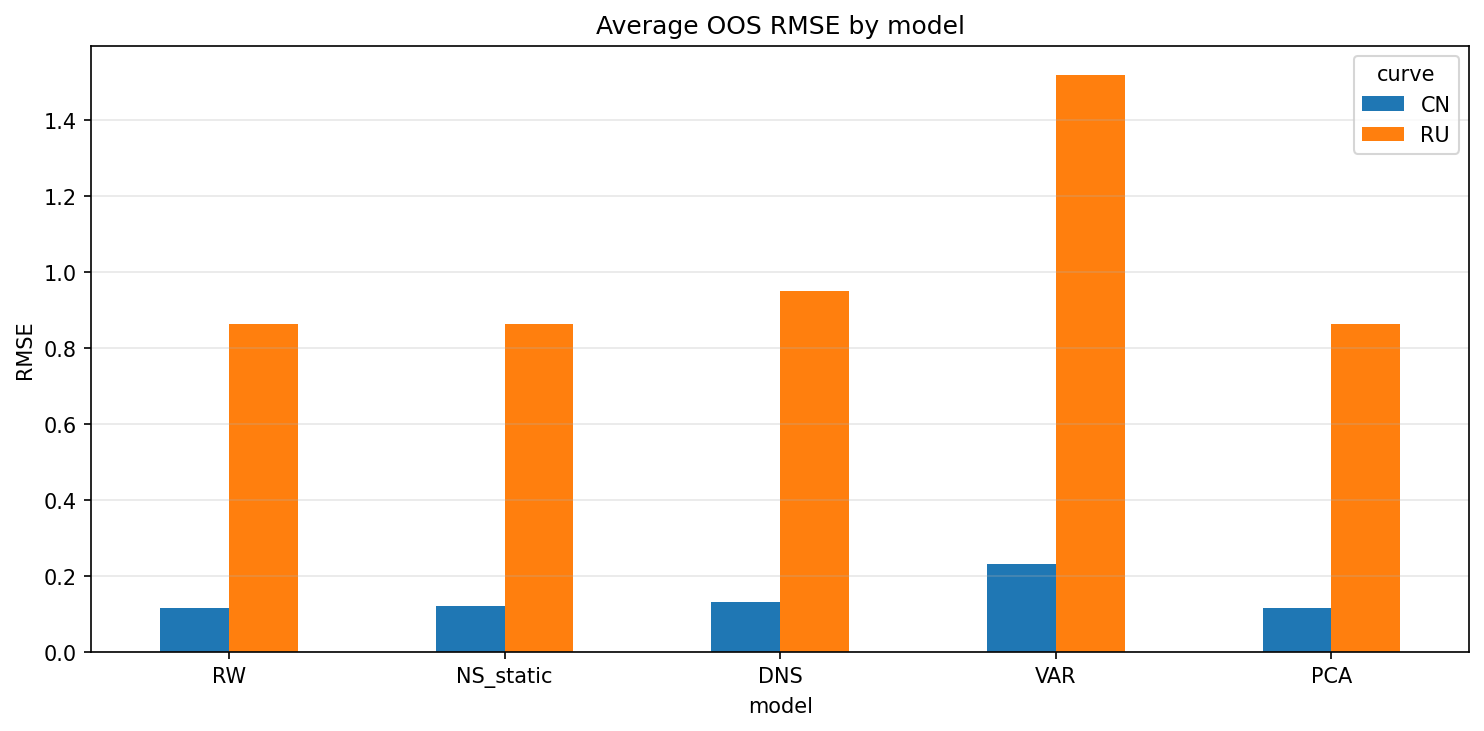
\includegraphics[width=0.75\textwidth]{tables/tab_6_3_model_comparison_avg_rmse.png}
\caption{Average OOS RMSE comparison from exported model-comparison artifacts.}
\label{fig:app_6_3_avg_rmse}
\end{figure}

\end{document}
